\chapter{Introduction to Lightning Network}

\label{Chapter05IntroLightning}

This Chapter provides the necessary background on the Lightning Network (LN) -- the main subject of this Part.
\footnote{This Chapter is partially based on~\cite{Tikhomirov2020a}.}
We review the history of payment channel protocols in Bitcoin and describe the architecture of the LN.


\section{Evolution of payment channels in Bitcoin}

Layer-two protocols allow blockchains to scale without modifying the core protocol (also referred to as \textit{layer-one} in this context).
This approach is also known as \textit{off-chain scaling}.
A layer-two protocol allows its two participants to exchange value without broadcasting every transaction to the blockchain.
Conflicts can be resolved on layer-one, hence preserving some if its security guarantees.

In the context of Bitcoin, layer-two protocols usually implement the concept of \textit{payment channels}.
A payment channel is a protocol that allows two parties to subsequently update the distribution of the initially committed funds.
Multiple ideas and implementations of Bitcoin payment channel have been proposed.
To put our work in historical context, we now describe the evolution of Bitcoin-based payment channels, following the outline in~\cite{BitcoinWikiChannels}.
See~\cite{McCorry2016} for an overview of Bitcoin payment channel designs.


\subsection{Transaction replacement with sequence numbers}

Satoshi Nakamoto proposed the first protocol for re-negotiating unconfirmed transactions.
This mechanism takes advantage of two Bitcoin features: transaction sequence number (\texttt{nSequence}) and time lock (\texttt{nLockTime}).
Each transaction has an \texttt{nSequence} field, which acts as a counter.
Originally, the protocol prescribed miners to prioritize transactions with higher sequence numbers, regardless of fees.
The time lock field (\texttt{nLockTime}) mandates a time before which a transaction cannot be confirmed in a block.
It is expressed either as a timestamp or as a block height.
The transaction replacement protocol prescribes the two parties to sign a series of transactions with increasing sequence numbers and a timelock at some point in the future.
The final state would be confirmed after the timelock expires.

The major drawback of this approach is that sequence numbers are not enforceable.
Miners have no economic incentives to prioritize a transaction with a higher sequence number, if it offers a lower fee than a conflicting transaction with a lower sequence number.
Miners even have a degree of plausible deniability: they may claim that they simply have not heard of the later transaction versions.
This may happen without malicious intent due to delays in the P2P network.


\subsection{Unidirectional channels}

Spillman channels, introduced in 2013, is the first version of unidirectional channels.
This protocol is a modified implementation of Nakamoto's transaction replacement protocol~\cite{Spillman2013}.
It has been implemented in BitcoinJ, a popular Bitcoin library written in Java~\cite{BitcoinJ}.

The channel participants are often described as a customer and a merchant.
Initially, they lock coins into a multi-signature output.
Additionally, they establish a time-locked refund transaction.
It allows the customer to withdraw all funds in case the merchant goes offline.
Then the customer signs a transaction that distributes the coins from the funding transaction in a new proportion, allocating more funds to the merchant.
The customer then sends the new transaction to the merchant. 
The merchant can either co-sign and broadcast it, thus closing the channel, or wait for the next transaction version.
Shortly before the timelock of the refund transaction expires, the merchant broadcasts the latest transaction.
This closes the channel and confirms the latest agreed upon balances.

This protocol has two major drawbacks.
First, it is unidirectional.
The customer can pay the merchant but not vice versa.
Second, the lifetime of a channel is limited by the timelock of the refund transaction.

A similar unidirectional payment channel design uses \texttt{CHECKLOCKTIMEVERIFY} (CLTV).
This opcode was added to Bitcoin script in 2015~\cite{Todd2014}.
It allows specifying absolute timelocks for each transaction output independently.
In contrast, \texttt{nLockTime} only described transaction-level timelocks.

\paragraph{State replacement}
Let us pause for a moment and explain why the protocols described so far do not support bidirectional payments.
Consider a channel between Alice and Bob.
Initially, Alice commits $10$~coins to a multi-signature address.
Thus, she has $10$~coins, and Bob has none.
Alice sends $2$~coins to Bob by signing a new transaction that spends the multi-signature output and distributes the coins as follows: $8$~coins to Alice, $2$~coins to Bob.
She sends this transaction to Bob.
However, Bob cannot send $1$~coin back to her.
If Bob were to sigh a new transaction that gives him $1$~coin, Alice would not accept it: she knows that he has another valid transaction that gives him $2$~coins.
Bob can therefore fraudulently broadcast that older transaction and effectively cancel his payment.

This issue is the key challenge in payment channel design.
It is known as the \textit{state replacement} problem.
Only the latest channel state should be valid.
In other words, only the last of multiple co-signed transactions should be accepted if broadcast to the blockchain.
All previous transactions, representing old channel states, must be provably invalidated.

The state replacement mechanism in unidirectional channels is referred to as \textit{revocation by incentive}~\cite{Gudgeon2019}.
Bob is \textit{incentivized} to close the channel using the last transaction, because that transaction gives him the largest amount of money.
To implement bi-directional channels, other state replacement mechanisms are required.


\subsection{Replace-by-timelock and Duplex channels}

Bidirectional channels can be implemented using timelocks.
The two parties exchange a series of transactions.
Each of them becomes valid at a point in time closer to the present than the previous transaction.
The transaction with the lowest time lock represents the latest state.
Any channel party can close the channel by submitting the latest state to the blockchain before other states become valid.
This protocol has two shortcomings.
First, similar to BitcoinJ's unidirectional channels, timelock-based bidirectional channels have a limited lifetime.
It is determined by the timelock of the first transaction.
Second, such channels only support a limited number of updates.
The delta between the timelocks of subsequent transactions must not be smaller than some security margin.
This ensures that each party can close the channel with the latest state before older states become valid.
Therefore, the maximum number of channel updates is determined by the channel lifetime and the minimal allowed difference between timelocks.
This type of state replacement is known as \textit{replace by timelock}.

Duplex micropayment channels~\cite{Decker2015} (DMC) implement bidirectional channels as a pair of unidirectional channels.
This protocol combines \textit{replace by timelock} and \textit{replace by incentive} state replacement.
The key concept of DMC is \textit{invalidation tree} -- a hierarchical transaction structure that allows for invalidation of old channel states.
Invalidation tree is based on the fact that the timelock of the first transaction in a chain defines the validity of all subsequent transactions.
A follow-up paper~\cite{Burchert2017} describes a way to share the cost of opening and closing channels among multiple parties.


\subsection{Poon-Dryja channels (Lightning)}

The Lightning Network (LN), proposed in 2016 by Poon and Dryja in~\cite{Poon2016}, overcomes the limitations of previous channel designs.
Lightning channels are \textit{bidirectional} and have an \textit{unlimited lifetime}.

The key insight in Lightning is its \textit{revocation-based state replacement}.
The transactions reflecting channel states are constructed in such a way that each next update \textit{invalidates} the previous one.
Despite the fact that all intermediate states are valid Bitcoin transactions (and can be broadcast and confirmed on the blockchain), broadcasting any state except the latest one by one party allows the other party to withdraw \textit{all} funds from the channel, punishing the cheater.

Lightning takes advantage of two relatively recent updates in Bitcoin.
One of them is \textit{relative timelocks}.
Contrary to earlier protocol, Lightning uses relative timelocks, as opposed to absolute ones.
A relative timelock makes a UTXO valid only after a certain time has passed after the transaction that created this UTXO is confirmed.
This functionality was implemented in BIP-112~\cite{BtcDrak2015} (\texttt{CHECKSEQUENCEVERIFY}) and activated in 2016.
An important advantage is that a transaction with a relative timelock may be signed but not broadcast for an indefinite period of time.
This allows Lightning channels to be left open indefinitely.
Let us now discuss the other Bitcoin update that made Lightning possible -- \textit{Segregated Witness}, or \textit{SegWit} -- in more detail.


\paragraph{Segregated witness}

Each transaction must specify the outputs it is spending.
An output is referenced by the \textit{hash} of the transaction and the \textit{index} of the output in that transaction.
In the initial versions of Bitcoin, the transaction hash was calculated based on all transaction data, including the signature.
The ECDSA signature scheme used in Bitcoin allows for multiple ways to sign the same message.
Consequently, one could abuse the signature malleability and sign the same transaction in different ways.
These would result in different transactions with equivalent semantics but different hashes.

Transaction malleability was a critical roadblock preventing the development of L2 protocols for Bitcoin.
A payment channels is generally initiated in three steps.
First, the parties co-sign the funding transaction that creates a multi-signature output.
Second, they co-sign a transaction that spends that output and reflect the initial distribution of funds.
Third, they confirm the funding transaction on the blockchain.

Note that the transaction created on step two refers to the output of the funding transaction, which is not yet broadcast.
Transaction malleability makes this step unreliable.
One of the parties may broadcast a modified version of the funding transaction, which has the same semantics but a different hash.
As a result, the original funding transaction would be become invalid~\cite{Harding2016}.

Additionally, transaction malleability complicates fraud prevention.
L2 protocols often assume that parties watch the blockchain for events of interest, such as broadcasts of old channel states.
With transaction malleability, the transaction hash does not uniquely define transaction semantics.
This issue makes watching the blockchain for relevant events hard, if not impossible.

SegWit, introduced in 2017, mitigated transaction malleability.
This update introduced a new category of transaction outputs, where the \textit{witness} (i.e.,~the signature) and other components of a transaction are \textit{segregated}.
As a result, the signature no longer affects the transaction hash, which mitigates the problem.
This opened the way for the practical implementation and deployment of more advanced Bitcoin-based L2 protocols.


\subsubsection*{Lightning development}

The development of the LN is guided by a set of documents called "Basics of Lightning Technology" (BOLTs)~\cite{BOLT}, which are then followed by several implementation teams.
The three most advanced implementations available in 2020 are LND~\cite{LND} (implemented in go), c-lightning~\cite{clightning} (implemented in C), and Eclair~\cite{Eclair} (implemented in Scala).
Other implementations at earlier stages of development include Electrum~\cite{ElectrumWebsite, ElectrumLightningAnnounce}, lit~\cite{lit}, lpd~\cite{lpd}, ptarmigan~\cite{ptarmigan}, and rust-lightning~\cite{rustlightning}.

As of 2020,~LN facilitates the off-chain exchange of more than $950$~BTC.
The protocol is under heavy development.
Lightning Network also operates with Litecoin~\cite{1MLLitecoin} -- an alternative cryptocurrency very similar to Bitcoin.

The future of Lightning depends in part on the planned modifications in the Bitcoin protocol.
Such changes usually take years to implement, test, and roll out.
Let us outline some of the directions for future developments of Lightning.

\paragraph{Schnorr-Taproot}

\textit{Schnorr signatures} is a digital signature algorithm that is considered preferable to ECDSA currently used in Bitcoin\footnote{Schnorr signature was covered by US patent~\cite{Schnorr1989}, which expired in 2008. This prevented its implementation in the original version of Bitcoin.}
In particular, this signature scheme allows for arithmetic on signatures.
In the context of Bitcoin, this allows for multi-signatures that are indistinguishable from signatures with a single signer.
Schnorr signatures are being integrated in Bitcoin as part of a complex \textit{Schnorr-Tapscript-Taproot} update~\cite{Hertig2020}.
For Lightning Network, Schnorr signatures allow for privacy improvements.
For instance, Lightning-related transactions indistinguishable from other transaction types from an external observer.

\paragraph{Eltoo}

\textit{Eltoo}\textit{Stylized as \textit{eltoo} in the original paper.} is an alternative payment channel proposal proposed by Decker, Russell, and Osuntokun in 2018~\cite{Decker2018}.
In Eltoo, intermediary transactions are linked to each other linearly, as opposed to the LN where all of them spend the same funding transaction output.
On channel closure, the final transaction is "re-attached" to the funding transaction's output.
This allows for more efficient state replacement.

Eltoo requires a new \textit{signature flag} -- \texttt{SIGHASH\_NOINPUT}~\cite{Decker2017}.
A signature flag specifies whether a transaction signature commits to all or only some of the inputs.
Allowing a transaction to \textit{not} commit to any input allows for "re-attaching" it to any compatible output.
If \texttt{SIGHASH\_NOINPUT} is deployed, this replacement mechanism can be used in LN or in a separate payment channel network.

\paragraph{Privacy-preserving channels}
A payment channel protocol called Bolt\footnote{Not to be confused with Basics of Lightning Technology (BOLT) -- the Lightning Network specification.} has also been proposed for a privacy-focused cryptocurrency Zcash~\cite{Green2017} and later modified for compatibility with Bitcoin and renamed to zkChannels~\cite{Akinyele2020}.



\section{Lightning Network architecture}
\label{sec:LightningOverview}

We now describe the key details of the Lightning Network protocol.

\subsection{Nodes}

Each \textit{LN node} is defined by an ECDSA private-public key pair.
A persistent \textit{node identifier} is derived from the hash of the public key. 
Additionally, the owner can assign a human-readable alias to their node.
Operations from a node are authorized with a digital signature created with the corresponding signing key.
One user can potentially own several nodes.

Nodes connect to each other in the P2P network identifying themselves by the IP address and the node ID.
Revealing the IP address is optional, but it is required if the node owner wants other nodes to be able to connect.
Nodes exchange information about the currently open channels and their fee policies.
Nodes communicate with an underlying bitcoin node (such as Bitcoin~Core) to receive information on the confirmed transactions.
\footnote{Some LN implementations partially support \textit{pruned} nodes~\cite{LNDInstall}.}


\subsection{Channels}

A \textit{payment channel} is a protocol for off-chain transactions.
A channel operates in three stages: opening (two parties lock the coins), operating (exchanging off-chain transactions), and closing (broadcasting the most recent channel state to the blockchain).


\subsubsection*{Channel opening}

Opening a channel consists of several steps.
To open a channel to Bob, Alice establishes a connection to Bob in the P2P network and issues a request to open a channel.
If the parties agree on channel parameters, they co-sign a \textit{funding transaction} that establishes the initial distribution of funds.
\footnote{While in the initial specifications~\cite{Poon2016} it was assumed that both parties could fund a channel, the current LN channels are single-funded: Alice provides all funds and may optionally "push" some funds to Bob as a gift.}.
The funding transaction creates a 2-of-2 multi-signature output that can be spent by Alice and Bob together if they agree to do so.

After the funding transaction gets the sufficient number of confirmations (usually~$3$~to~$6$), the channel is open.
The capacity of the channel is determined by the amount of coins deposited when created and stays constant during its lifetime.
\footnote{Not accounting for LN fees.}

\subsubsection*{Channel updates}

An \textit{LN transaction} is an atomic update of one or multiple channels.
In single channel updates, two users agree on an updated balance.
In multi-hop transactions, the balances of several channels forming a path are simultaneously updated.

\paragraph{Single-channel transactions}

To send a payment to Bob, Alice negotiates a new channel state.
Each channel state is reflected in a \textit{commitment transaction}.
A commitment transaction spends the output of the funding transaction and re-distributes the coins between Alice and Bob.

More precisely, each channel state is encoded in a \textit{pair} of commitment transactions: one for Alice and one for Bob.
These transactions are symmetric: they enforce a timelock on the party that holds the transaction.
In particular, Alice's version of commitment transactions allow her to redeem her output only after a timeout.
Bob's version imposes analogous restrictions on his output.
This enables the state replacement mechanism (described below), which provides economic security guarantees to LN channels, assuming the parties are watching the blockchain sufficiently often.

Outputs of commitment transactions are called \textit{Hash time-locked contracts}, or \textit{HTLC}s.
%An HTLC gives the funds either to one party, if it provides a preimage of a given hash, or to the other party after a timeout.
An HTLC allows a node ($u_1$) to lock $x$~coins in a channel between two nodes ($u_1$~and $u_2$) and release them according to the encoded conditions.
The terms for the HTLC($u_1, u_2, y, x, t$) are defined with a hash value $y := H(r)$, an amount $x$~of coins, and a timeout $t$, as follows: 
(i) If $u_2$~reveals a value $r$~such that $H(r) = y$~before $t$~expires, $u_1$~pays $x$~to $u_2$; 
(ii) if $t$~expires, $u_1$~receives $x$~back.

A simple LN payment proceeds as follows.
If Alice wants to send $x$~coins to Bob, she first asks him for a \textit{payment hash}.
Bob generates $r$~uniformly at random and sends its hash $H(r)$~to Alice in an \textit{invoice} message.
Alice then \textit{offers} Bob an HTLC that can be \textit{resolved} in one of two ways.
Either Bob reveals $r$~and \textit{redeems} the coins before time $t$, or Alice gets the coins back.
A payment channel can keep track of multiple concurrent unresolved HTLCs, which are also called \textit{in-flight} HTLCs.


\paragraph{Multi-channel transactions}

\begin{figure*}[h]
	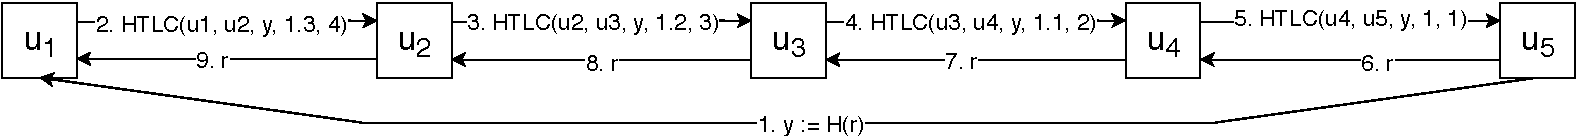
\includegraphics[width=\textwidth]{htlc-figure}
	\caption{An HTLC-based payment in the LN. The node $u_1$~pays $u_5$~using $u_2$, $u_3$~and $u_4$~as intermediaries. 
		Here we assume that each node charges a fee of $0.1$~and time is measured in days.}
	\label{fig:htlc}
\end{figure*}

A multi-channel transaction leverages a path of channels between a sender and a receiver, who might not share a channel between them.
To initiate a multi-channel transaction, the receiver generates a random $r$~and sends its hash $H(r)$~to the sender.
The sender then constructs a path to the receiver and sets up an HTLC with the next node in the path.
The second node sets up an HTLC with the \textit{same} hash value with the third node, and so on.
Finally, the receiver redeems the payment from the last channel by revealing $r$, which in turn allows all involved channels to be updated.

Note that all HTLCs along the path use the same hash value $y=H(r)$.
This aims to achieve atomicity.
None of the intermediate channels can be updated before the receiver reveals $r$, and all of them can be updated after that.

An illustrative example of an HTLC-based transaction is depicted in~\cref{fig:htlc}.
Here, the user $u_1$~transfers $1$~coin to $u_5$~using $u_2$, $u_3$~and $u_4$~as intermediaries.
For that, $u_5$~locally chooses a value $r$~uniformly at random, computes the cryptographic challenge for the HTLC as $y := H(r)$, and sends $y$~to the sender in an \textit{invoice} (step 1).
Then, the payment starts with a commit phase (steps 2-5) where every pair of nodes, starting from the sender, establishes an HTLC using $y$.
After the commit phase is finished, the transaction enters the release phase.
Here, the receiver reveals $r$~to $u_4$~to fulfill the contract (step 6), triggering the release phase where every pair of nodes fulfills their contract from the receiver to the sender (steps 6-9).

Intermediaries may charge fees for their forwarding service.
For instance, $u_2$~receives $1.3$~coins but only forwards $1.2$~coins, getting a fee of $0.1$~coins.
No fees are collected if a payment fails, as all pending balance updates roll back.
In the actual LN protocol, the fee consists of two parts: a constant \textit{base fee} for each payment and a \textit{fee rate} proportional to the value being transferred.
\footnote{Note that LN fee structure is different from fees on L1, where the fee is proportional to transaction weight (roughly speaking, size in bytes) but does not account for the amount of value being transferred. This may result in the economics of LN fees being significantly different from that in Bitcoin. As of 2020, LN fees are largely non-economical~\cite{Beres2019}.}

Note that the time parameter of the HTLCs along the path is decreasing to ensure a safety margin between the timeouts.
For example, the HTLC between $u_1$~and $u_2$~sets a timeout of four days, whereas the timeout in the HTLC between $u_2$~and $u_3$~is only three days.
This ensures that $u_2$~has enough time to settle the contract with $u_1$~after receiving $r$~from $u_3$, even if $u_3$~reveals the preimage just before the corresponding timeout expires.
There is an inherent trade-off regarding timeout lengths.
Short timeouts open the risk of not being able to dispute a fraudulent transaction in case of blockchain congestion.
Long timeouts open up a DoS vector, where an attacker can route many unsettled payments through a channel and effectively block it until the timelock expires.

Multi-path payments use onion routing to enforce the order of intermediary nodes.
Each intermediary node only knows the immediate previous and next nodes, but not the final sender or receiver and not its position in the path.


\subsubsection*{Channel closure}

A channel is closed when a transaction that spends the output of the funding transaction gets confirmed on-chain.
This may happen in one of three ways:

\begin{itemize}
	\item Collaborative closure. Alice signals the intent to close the channel, and Bob cooperates in signing the transaction that reflects the latest channel state. This results in one on-chain transaction to close a channel, and no delays for both parties. Both parties must be online and cooperating.
	\item Non-cooperative closure without breach. Alice signals the intent to close the channel, but Bob does not respond. In this case, Alice publishes the latest commitment transaction on the blockchain. Bob can redeem his output immediately, but Alice has to wait until a timeout expires. This is a safety measure to provide Bob with an opportunity to broadcast a \textit{justice transaction} (see below).
	\item Non-cooperative closure with breach. Alice broadcasts an old commitment transaction in an attempt to close the channel with an outdated channel state (thus potentially stealing from Bob). If Bob does not react before the timelock on Alice's output expires, Alice can redeem her output, and the channel is closed.\footnote{From the on-chain point of view, a non disputed non-cooperative close is indistinguishable from a non-cooperative close without a breach. Layer-one does not know whether a commitment transaction is the last one, unless this fact is disputed.} If Bob is online and notices the breach before the timeout, he broadcasts the latest commitment transaction, which allows Bob to spend Alice's output before she can, punishing her for the cheating attempt.
\end{itemize}

This state replacement mechanism is the key element of LN, which makes it superior to earlier payment channel designs.
Lightning channels have an unlimited lifetime (the parties do not have to close the channel if none of them wants to) and supports payments in both directions.
However, there is a trade-off here: the parties must be online to notice potential malicious channel closures and broadcast justice transactions.
This functionality can be outsourced.
Entities that watch the blockchains for malicious channel closures and dispute them on behalf of a user are called \textit{watchtowers}.
Implementing effective, economically incentivized, and privacy-preserving watchtowers in an active area of research~\cite{McCorry2019}.

LN's revocation technique has proved effective as a deterrence against malicious channel closures.
As of July~2019, there has been only $241$~channel closures followed by a justice transaction.
This constitutes only $0.7$\%~of channels at that time~\cite{BitMEXLN3}.
\footnote{The research is based on the LN's on-chain footprint and is not absolutely accurate. A non-cooperative closure followed by a justice transaction may also happen without malicious intent, for example, as a result of a broken backup restore (where Alice's node "forgets" about the latest state and broadcasts an earlier state assuming it is the latest one).}


\subsection{P2P network and path-finding}

Lightning network is \textit{source-routed}: the sender determines the path to the receiver.
But how does the sender construct such a path?

LN nodes gossip about newly opened channels that are marked as available for routing.
Based on this information, each node maintains a local model of the network graph, and uses it to generate routes to the receiver.
Total capacities of public channels are known.
Therefore, the sender only considers channels with the capacity larger than $x$~for a payment of amount $x$.

However, this is insufficient to prevent routing failures.
The ability of channel parties to send or forward payments is limited by their \textit{local} channel balances.
Consider an example.
After Alice opens a channel with Bob, all funds are initially on her side.
This means that she can send up to the total capacity, but she can not receive.
As the local balances change, the routing capabilities of the channel in both directions also change.

The fact that local channel balances are not public makes routing unreliable, especially for larger amounts.
If a payment fails, an error message notifies the sender which channel has failed.
The sender then tries a different route.
The process repeats until the payment succeeds.
Optimizing path-finding for payment channel networks is an active area of research~\cite{Pickhardt2019a, Prihodko2016, Grunspan2018, Pickhardt2019, Piatkivskyi2018, Sivaraman2018, Bagaria2019, Roos2018}.
